\documentclass{article}

%% doc settings
\hyphenchar\font=-1 % suppress hyphenation
\setlength\parindent{0pt} % suppress indentation
\usepackage[margin=1.5truein]{geometry} % set page margins

\usepackage{listings}
\usepackage{lastpage}
\usepackage{fancyhdr}
\usepackage{amsmath}
\usepackage{amssymb}
\usepackage{url}
\usepackage{xcolor}
\usepackage{graphicx}
\usepackage{hyperref}
\usepackage{enumitem}
\usepackage{tikz}
\usepackage{forest}
\usetikzlibrary{trees,positioning,shapes,shadows,arrows.meta}

\graphicspath{{./}}

\hypersetup{
    colorlinks = true,
    linkcolor = red,
    urlcolor = red
}

\definecolor{codegreen}{rgb}{0,0.6,0}
\definecolor{codegray}{rgb}{0.5,0.5,0.5}
\definecolor{codepurple}{rgb}{0.58,0,0.82}
\definecolor{backcolour}{rgb}{0.95,0.95,0.92}

\lstdefinestyle{mystyle}{
    backgroundcolor=\color{backcolour},   
    commentstyle=\color{codegreen},
    keywordstyle=\color{magenta},
    numberstyle=\tiny\color{codegray},
    stringstyle=\color{codepurple},
    basicstyle=\ttfamily\footnotesize,
    breakatwhitespace=false,         
    breaklines=true,                 
    captionpos=b,                    
    keepspaces=true,                 
    numbers=left,                    
    numbersep=5pt,                  
    showspaces=false,                
    showstringspaces=false,
    showtabs=false,                  
    tabsize=2
}

\lstset{style=mystyle}

%% page nums
\pagestyle{fancy}
\fancyhf{}
\fancyfoot[C]{Pg. \thepage \space of \pageref*{LastPage}}
\renewcommand{\headrulewidth}{0pt}

%% begin doc
\begin{document}
\title{SYSEN 6150: Model Based Systems Engineering\\~\\
    \Large Customer Affinity Process, Design Review Reaction, \\
    Annotated Concept Sketch
}
\author{
    Nick Kunz [NetID: \url{nhk37}] \hyperlink{nhk37@cornell.edu}{nhk37@cornell.edu}}
\date{September 9, 2022}
\maketitle
\thispagestyle{fancy}

\section*{Customer Affinity Process}
The following exhibits a Customer Affinity Process for the core development of PyTorch.
PyTorch is an open source machine learning framework for experimential use and production.
Below are 10 brief examples of user/customer requests that have been labeled according to their use within \textit{production}.
In the case where more examples of user/customer requests were included, an additional label would likely emerge containing features related to \textit{experiments}, where an even broader label would likely emerge to combine them.

\tikzset{
  basic/.style  = {draw, text width=2cm, drop shadow, font=\sffamily, rectangle},
  root/.style   = {basic, rounded corners=6pt, thin, align=center, fill=white, text width=6cm},
  level-2/.style = {basic, rounded corners=6pt, thin,align=center, fill=white, text width=3cm},
  level-3/.style = {basic, align=left, fill=white, text width=12cm}
}

\begin{figure}[htbp]
\centering
\begin{tikzpicture}[
    level 1/.style={sibling distance=12em, level distance=5em}, 
    {edge from parent fork down},
    edge from parent/.style={->,solid,black,thick,sloped,draw},
    edge from parent path={(\tikzparentnode.south) -- (\tikzchildnode.north)},
    >=latex, node distance=1cm, edge from parent fork down
]

% root of the the initial tree, level 1
\node[root]{\textbf{PyTorch Production}}
% The first level, as children of the initial tree
    child {node[level-2] (c1) {\textbf{ONNX}}}
    child {node[level-2] (c2) {\textbf{Tensors}}}
    child {node[level-2] (c3) {\textbf{Tests}}};

% The second level, relatively positioned nodes
\begin{scope}
\node [below of = c1, xshift=4em] (c11) {Change symbolic func.};
\node [below of = c11] (c12) {Use type guard value.};
\node [below of = c12] (c13) {Improve model export.};

\node [below of = c2, xshift=4em] (c21) {INT32 not working.};
\node [below of = c21] (c22) {Change tensor list.};
\node [below of = c22] (c23) {Increase profilings.};
\node [below of = c23] (c24) {Support for nvFuser.};
\node [below of = c24] (c25) {Dispatch GPU pooling.};

\node [below of = c3, xshift=4em] (c31) {Debug error 1.12.1.};
\node [below of = c31] (c32) {OpInfo test comps.};
% \node [below of = c32] (c33) {item 3-3};
% \node [below of = c33] (c34) {item 3-4};
% \node [below of = c34] (c35) {item 3-5};
\end{scope}

% lines from each level 1 node to every one of its "children"
\foreach \value in {1,...,3}
  \draw[->] (c1.195) |- (c1\value.west);

\foreach \value in {1,...,5}
  \draw[->] (c2.195) |- (c2\value.west);

\foreach \value in {1,...,2}
  \draw[->] (c3.195) |- (c3\value.west);
  
\end{tikzpicture}
    \caption{Customer Affinity Process}
    \label{fig:tax}
\end{figure}

\newpage
\section*{Design Review Reaction}

\textbf{Mindstorm Robotics Challenge: Team 2 (Alphaverse)}\\~\\

\noindent
On Wednesday, August 31th, 2022 at 11:00AM EST, Team 2 (Alphaverse), conducted a design review for the Mindstorm Robotics Challenge. The team was represented by Amal Bhaskaran, under the supervision of the assumed \textit{“boss”}, David R. Schneider.\\~\\
The team revealed several strengths and weaknesses during the conversation. The two main strengths were: 1) they had implemented intermediate deadlines nested within the broader project completion time, and 2) they were open to both structural and functional critique and welcomed feedback if it meant that it would help solve the customers problem.\\~\\
Although the project demonstrated a clear direction, the team still had ways in which they could improve. The two main weaknesses they exhibited were: 1) they recast the problem into a solution too quickly - that is to say, the team relied too heavily on structural explanations and quickly arrived at a solution, rather than first addressing the customer's functional requirements, and 2) they lacked a baseline of performance halfway through the development cycle.\\~\\
At this time, it seems like the team would benefit most from continuing their practice and development of intermediate deadlines and being open to feedback from the customer and leadership, while at the same time revisiting many of the functional concerns of the customer to ensure that their structural solutions met those requirements. In addition, it would be beneficial for the team to conduct a number of tests to establish a baseline of performance that they could improve upon in what time they still have to develop their robot.\\~\\

\newpage
\section*{Annotated Concept Sketch}

The following exhibits both \textit{structural} and \textit{functional} annototated concept sketches for a Fortin Barometer.
A Fortin Barometer measures atmospheric pressure utilizing a column of mercury. 
Below are 6 features of the instrument, each outlined according to their respective categories.

\begin{figure}[!ht]
    \centering
    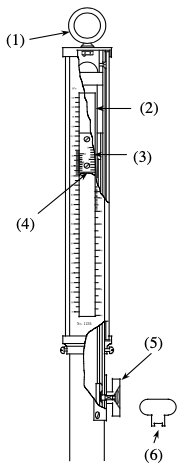
\includegraphics[height=9cm]{fortin.png}
    \caption{Fortin Barometer (1)}
    \label{fig:baro}
\end{figure}
\textbf{Figure 2: Structural Annotations}
\begin{enumerate}[itemsep=-0.5em]
    \item External grasping ring.
    \item Extended pressure scale.
    \item Scale containing multiple measurements.
    \item Extra wide mercury column.
    \item Calibration knob.
    \item Rough adjustment tool.
\end{enumerate}

\textbf{Figure 2: Functional Annotations}
\begin{enumerate}[itemsep=-0.5em]
    \item Fastener for suspending device from a fixed position.
    \item Device can measure high increases in pressure.
    \item Pressure can be read in either hPa or atm.
    \item Easy to read and record measurements.
    \item Easy to calibrate in the field.
    \item Prevent rough tuning from fielded device.
\end{enumerate}

\newpage
\section*{References}

1. World Meteorological Organization (WMO), “Figure 5.2: Structure of the Fortin Barometer,” \textit{in Chapter 5: Measurement of Atmospheric Pressure, WMO Training Workshop for RA II Instrument Specialists.} Tsukuba, Japan: Japan Meteorological Agency (JMA), 1998, pp. 2. 

\end{document}